% To je predloga za poročila o domačih nalogah pri predmetih, katerih
% nosilec je Blaž Zupan. Seveda lahko tudi dodaš kakšen nov, zanimiv
% in uporaben element, ki ga v tej predlogi (še) ni. Več o LaTeX-u izveš na
% spletu, na primer na http://tobi.oetiker.ch/lshort/lshort.pdf.
%
% To predlogo lahko spremeniš v PDF dokument s pomočjo programa
% pdflatex, ki je del standardne instalacije LaTeX programov.

\documentclass[a4paper,11pt]{article}
\usepackage{a4wide}
\usepackage{fullpage}
\usepackage[utf8x]{inputenc}
\usepackage[slovene]{babel}
\selectlanguage{slovene}
\usepackage[toc,page]{appendix}
\usepackage[pdftex]{graphicx} % za slike
\usepackage{setspace}
\usepackage{color}
\definecolor{light-gray}{gray}{0.95}
\usepackage{listings} % za vključevanje kode
\usepackage{hyperref}
\usepackage{float}
\usepackage{verbatim}
\renewcommand{\baselinestretch}{1.2} % za boljšo berljivost večji razmak
\renewcommand{\appendixpagename}{Priloge}

\lstset{ % nastavitve za izpis kode, sem lahko tudi kaj dodaš/spremeniš
language=Python,
basicstyle=\footnotesize,
basicstyle=\ttfamily\footnotesize\setstretch{1},
backgroundcolor=\color{light-gray},
}

\title{Šesta domača naloga}
\author{Anže Pečar (63060257)}
\date{\today}

\begin{document}

\maketitle

\section{Uvod}
Namen "seste doma"ce naloge je seznaniti se s podatki za tekmovanje iz podro"cja kemoinformatike. 

\section{Podatki in opis problemske domene}
Problemska domena ima $1776$ atributov in $3751$ primerov. Vrednosti atributov so med 0 in 1. Najbolj pogostih 5 vrednosti atributov je zapisanih v tabeli \ref{pt}.

\begin{table}[htbp]
\caption{Najbolj pogoste vrednosti atributov.}
\label{pt}
\begin{center}
\begin{tabular}{llp{3cm}}
\hline
vrednost atributa & "st ponovitev \\
\hline
0.0 & 5593148 \\
1.0 & 421473 \\
0.125 & 20583 \\
0.1667 & 17677 \\  
0.25 & 17127 \\
\hline
\end{tabular}
\end{center}

\end{table}



%"St razli"cnih vrednosti za posamezen atribut je v logaritemski skali prikazano na sliki \ref{atrs}.

%\begin{figure}[H]
%\begin{center}
%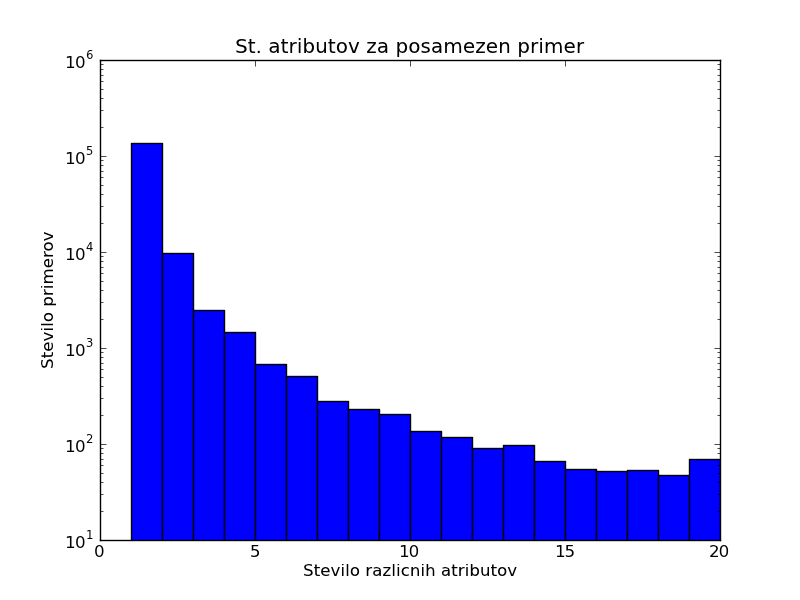
\includegraphics[scale=0.3]{atrs.png}
%\caption{"St. razli"cnih vrednosti atributov}
%\end{center}
%\label{atrs}
%\end{figure}

Ve"cina atributov ima eno ali dve razli"cni vrednosti. Kar precej ($836$) atributov ima samo dve razli"cni vrednosti in bi jih lahko smatrali za diskretne atribute. "Ce bi za diskretne atribute vzeli atribute, ki imajo 5 razli"cnih vrednosti, bi imeli $1095$ diskretnih in $681$ zveznih atributov.

\section{Informativnost atributov}

Za izra"cun informativnosti sem uporabil Orangeovo implementacijo Reliefa. Relief mi je za 3 najbolj informativne atribute izbral D27 ($0.2145$), D1036 ($0.1368$), D961 ($0.1313$). 

Relief ocenjuje kvaliteto atributov glede na to, kako dobro lo"cujejo posamezne razrede. Za vsak primer Relief poi"s"ce dva najbli"zja soseda; enega iz istega razreda (najbli"zji zadetek) in enega iz razli"cnega razreda (najbli"zja zgre"sitev). "Ce imata dva primera razli"cni vrednosti najbli"zjega zadetka atributa, potem ta atribut lo"cuje dve instanci z istim razredom, kar ni za"zeljeno in se zato vrednost tega atributa zmanj"sa.

Algoritem relief ra"cuna razliko med dvema diskretnima atributoma po formuli:

\[ diff(A, I_1, I_2) = \left\{
	\begin{array}{ll}
		0  & if value(A,I_1) == value(A, I_2) \\
		1 & drugace
	\end{array}
\right. \]

Za zvezne atribute pa ra"cuna po formuli:

\[ diff(A, I_1, I_2) = \frac{\vert value(A,I_1) - value(A, I_2) \vert}{max(A) - min(A)} \]

kjer je A izbran atribut, $I_1$ in $I_2$ pa dva primera (instanci). Formuli sem povzel po "clanku \cite{relief}

Katere atribute upo"stevati je mo"cno odvisno od modela, ki ga uporabimo za u"cenje. Preizkusil sem ve"c razli"cnih pragovnih vrednosti z razli"cnimi modeli. Pri naklju"cnih drevesih sem dobil najbolj"si rezultat pri pragu $0.0$, knn pa pri pragu $0.1$. 



\section{Ocenjevanje kakovosti napovednih modelov}

Za napovedovanje sem uporabil tri kvalifikacijske algoritme, ki so vklju"ceni v Orangeovi knji"znici - RandomForest, kNN in NaivniBayes. Algoritme sem preizkusil z 10 kratnim pre"cnim preverjanjem, rezultati pa so podani v tabeli \ref{rez}.

\begin{table}[htbp]
\caption{Rezultati 10 kratnega pre"cnega preverjanja}
\label{rez}
\begin{center}
\begin{tabular}{llp{3cm}}
\hline
algoritem & log loss ocena \\
\hline
RandomForest & 0.464369549067 \\
kNN & 0.536824035629 \\
NaivniBayes & 0.627878923437\\
\hline
\end{tabular}
\end{center}
\end{table}

Na lestvici vode"cih bi se z najbolj"sim rezultatom (RandomForest) uvrstili na 150. mesto. To je dober za"cetek, ampak za bolj"si rezultat bo potrebno implementirati stackanje algoritmov. 

\section{Izjava o izdelavi domače naloge}
Domačo nalogo in pripadajoče programe sem izdelal sam.


\begin{thebibliography}{9}

\bibitem{relief}
   Ian H. Witten \& Eibe Frank,
   \emph{Theoretical and Empirical Analysis of ReliefF and RReliefF}
   Marko Robnik-Sikonja, Igor Kononenko,
   2003.

\end{thebibliography}

\end{document}
